\documentclass[11pt]{article}
\usepackage[utf8]{inputenc}
\usepackage[T1]{fontenc}
\usepackage[margin=1in]{geometry}
\usepackage{amsmath,amssymb}
\usepackage{authblk}
\usepackage{graphicx}
\usepackage{enumitem}
\usepackage{xcolor}
\usepackage{hyperref}
\hypersetup{colorlinks=true,linkcolor=blue!50!black,citecolor=blue!50!black,urlcolor=blue!50!black}
\usepackage{listings}
\lstset{basicstyle=\ttfamily\small,breaklines=true,columns=fullflexible}
\usepackage{tikz}
\usetikzlibrary{arrows.meta,positioning,fit,backgrounds}
\usepackage{pgfplots}
\pgfplotsset{compat=1.18}
\usepackage{booktabs}
\usepackage{multirow}
\usepackage{array}
\usepackage{titlesec}
\titlespacing*{\section}{0pt}{1.4em}{0.7em}
\titlespacing*{\subsection}{0pt}{1.1em}{0.5em}
\setlength{\parskip}{0.4em}
\setlength{\parindent}{0pt}

\title{\textbf{TPM-Attest: Hardware-Rooted Integrity Attestation as a Kernel-Level Anti-Cheat Alternative for Linux}}

\author[1]{Anudeep Gedela}
\author[1,*]{Dr.\ A.\ Yaswanth}
\affil[1]{GITAM School of Technology, GITAM (Deemed to be University), Visakhapatnam, India}
\affil[*]{Corresponding author -- Assistant Professor, Department of Computer Science \& Engineering, \texttt{yamanapu@gitam.edu}}
\date{}

\begin{document}
\maketitle

\begin{abstract}
Linux gaming and remote host verification are historically constrained by proprietary, high-privilege kernel-level software (e.g., Easy Anti-Cheat, BattlEye). These modules require Windows-centric Ring~0 privileges or unstable Linux kernel modules, raising significant security, stability, and licensing concerns. We propose \textbf{TPM-Attest}, a hardware-rooted remote attestation framework leveraging Trusted Platform Modules (TPM)~2.0 and the Linux Integrity Measurement Architecture (IMA). TPM-Attest proves system-wide platform and software execution integrity from the hardware level without requiring high-privilege active memory scanners. Our implementation comprises a client-side TPM attestation agent, an IMA-based Merkle tree verifier immune to leaf-collision attacks, a FastAPI verification server with an SQLite persistence layer, and a dynamic userspace \texttt{LD\_PRELOAD} hook gating game sessions by intercepting Epic Online Services (EOS) SDK calls. Experimental evaluation across 500 attestation sessions demonstrates a 100\% tamper-detection rate for binary substitution, IMA log truncation, and nonce replay, with incremental repeat-attestation latency under 3~seconds. We compare TPM-Attest against Keylime and commercial kernel-mode anti-cheat baselines across security, performance, and deployability dimensions, and provide a comprehensive threat-model analysis with supporting statistical results.
\end{abstract}

\section{Introduction}
\label{sec:intro-ref}

Personal computer gaming on Linux has undergone a massive transformation, driven by compatibility layers like Valve's Proton~\cite{valve2018proton}. However, multiplayer PC gaming remains restricted on Linux because proprietary kernel-space anti-cheat modules (operating in Ring~0 on Windows) are incompatible with the Linux security model and GPL licensing. On Linux, the absence of a stable kernel ABI means proprietary drivers cause frequent system instability. Moreover, executing un-auditable, proprietary binaries at the kernel level introduces severe local privilege escalation vectors; a recent independent examination of four widely deployed kernel-level anti-cheat systems found that two exhibited rootkit-like properties, including broad, unrestricted OS visibility exceeding what their stated purpose requires~\cite{dorner2024rootkit}.

This paper proposes replacing invasive, active runtime memory scanning with \textbf{passive, hardware-rooted remote attestation}. By utilizing the Trusted Platform Module (TPM)~2.0 microcontroller present on modern motherboards, we cryptographically verify that the client system booted into a trusted state and executed only authorized binaries~\cite{tcg2018}.

By anchoring the Linux kernel's Integrity Measurement Architecture (IMA) to the TPM, we generate a hardware-secured, append-only log of every binary, library, and kernel module loaded since boot~\cite{sailer2004ima}. When a client requests access, it must present a hardware-signed TPM quote containing the system state (Platform Configuration Registers or PCRs) and the runtime execution log. A remote verifier validates the signature and checks the log against a pinned baseline before issuing a short-lived cryptographically signed session token~\cite{rats2023}. We demonstrate this paradigm end-to-end using a dynamic hook to intercept SDK connections and gate game play on attestation results.

The key contributions of this paper are:
\begin{enumerate}[nosep]
  \item An open-source, end-to-end TPM-Attest framework combining TPM~2.0 quotes and IMA measurement logs for Linux gaming integrity verification.
  \item An index-prefixed Merkle tree construction immune to duplicate-leaf collision attacks (CVE-2012-2459 class).
  \item A dynamic \texttt{LD\_PRELOAD} interception hook gating EOS SDK sessions on real-time attestation results.
  \item A comprehensive experimental evaluation including latency profiling, tamper-detection rates, and a comparative analysis against Keylime and kernel-mode anti-cheat baselines.
  \item \textbf{VOID SECTOR} -- a complete playable 2-D space-shooter demo game whose session launch is gated end-to-end by the TPM-Attest pipeline, providing a live, reproducible demonstration of the full attestation flow (game client $\to$ hook $\to$ daemon $\to$ TPM $\to$ server $\to$ session granted/denied).
\end{enumerate}

\section{Background and Foundations}

\subsection{TPM 2.0 and Platform Configuration Registers (PCRs)}
The TPM~2.0 microcontroller operates as a secure cryptoprocessor physically isolated from the host CPU~\cite{tcg2018}. Platform Configuration Registers (PCRs) are volatile memory slots storing hashes representing the platform's boot and software state. PCRs are updated via a one-way \textbf{extend} operation:

\begin{equation}
  \text{PCR}_{\text{new}} = \text{SHA-256}\!\left(\text{PCR}_{\text{old}} \,\|\, m\right)
  \label{eq:pcr-extend}
\end{equation}

\noindent where $m$ is the new measurement value. This one-way chaining prevents register rollback or state forging. A TPM quote (\texttt{tpm2\_quote}) extracts a signed digest of selected PCRs using an asymmetric Attestation Key (AK), incorporating a caller-supplied challenge nonce $\eta$ to guarantee freshness~\cite{tpm2tools2024}.

\subsection{Integrity Measurement Architecture (IMA)}
Linux IMA is a kernel subsystem that intercepts system calls mapping files for execution (e.g., \texttt{execve}, \texttt{mmap})~\cite{lko2021}. It computes file hashes, appends them to an in-memory ASCII log, and extends the measurements into PCR~10. The log is anchored by the \texttt{boot\_aggregate} measurement (representing PCRs 0--7), linking runtime executions to the physical boot state. The aggregate is defined as:

\begin{equation}
  \texttt{boot\_aggregate} = \text{SHA-256}\!\left(\bigoplus_{i=0}^{7} \text{PCR}_i\right)
  \label{eq:boot-agg}
\end{equation}

\subsection{Shared Library Interception (\texttt{LD\_PRELOAD})}
On Unix systems, the dynamic linker allows loading custom shared libraries before standard dependencies via the \texttt{LD\_PRELOAD} environment variable~\cite{kerrisk2010}. By exporting matching function symbols (such as those in the Epic Online Services SDK), we intercept SDK network calls at runtime, evaluate local attestation status, and block access transparently.

\subsection{Index-Prefixed Merkle Tree}
Standard binary Merkle trees are susceptible to duplicate-leaf collision attacks~\cite{bitcoin2012cve}. TPM-Attest prevents this by prepending the absolute log index $i$ to the leaf hash preimage:

\begin{equation}
  \ell_i = \text{SHA-256}\!\left(i \,\|\, \text{pcr}_i \,\|\, \text{tmpl\_hash}_i \,\|\, \text{file\_hash}_i \,\|\, \text{filename}_i\right)
  \label{eq:leaf}
\end{equation}

Internal nodes are computed as:
\begin{equation}
  n_{\text{parent}} = \text{SHA-256}\!\left(\ell_{\text{left}} \,\|\, \ell_{\text{right}}\right)
  \label{eq:internal}
\end{equation}

Since $\ell_i$ is bound to its absolute position $i$, duplication or reordering changes the leaf hash and is rejected by the verifier.

\section{Related Work}
\label{sec:related-work}

Hardware-rooted remote attestation using TPM measurements has a long research history. Sailer et al.\ introduced IMA, showing a remote verifier could detect compromised binaries on a running Linux host~\cite{sailer2004ima}. \textbf{Keylime}, originally built at MIT Lincoln Laboratory and now a CNCF project, combines TPM quotes and IMA logs into an agent/registrar/verifier architecture for cloud, edge, and IoT device attestation~\cite{keylime}. TPM-Attest adopts a similar measurement pipeline but targets a different deployment point: it gates a single consumer desktop's game session at process-launch time and integrates directly with the EOS SDK through an \texttt{LD\_PRELOAD} hook.

Dorner and Klausner's 2024 analysis of four widely deployed kernel-level anti-cheat systems found that two exhibited rootkit-like behavior~\cite{dorner2024rootkit}. TPM-Attest responds directly to this finding by removing the kernel-mode component entirely. Alangari and Alharbi's 2025 systematic review categorizes existing defenses and notes a persistent trade-off between kernel-level visibility and privacy/stability risk~\cite{alangari2025review}. Coker et al.\ presented principles for remote attestation that align with our challenge-response nonce protocol~\cite{coker2011principles}. Bratus et al.\ analyzed the limitations of trust-measurement pipelines against adversaries with privileged access~\cite{bratus2008}. Petroni et al.\ examined copilot-based hardware rootkit detection, highlighting that passive measurement complements active scanning~\cite{petroni2004}.

\section{Threat Model and Security Goals}
\label{sec:threat-model}

\subsection{Adversary Capabilities}
We assume a motivated adversary with administrative (root) access to the host OS. The adversary aims to load modified game binaries, inject dynamic cheat libraries, or bypass anti-cheat mechanisms. They are capable of:
\begin{itemize}[nosep]
  \item Modifying binaries on disk or injecting libraries at runtime.
  \item Loading custom, unsigned kernel modules.
  \item Intercepting and replaying attestation reports.
  \item Spawning game clients inside VMs with software-emulated TPMs.
\end{itemize}

\subsection{Prevented Attacks}
\begin{enumerate}[nosep]
  \item \textbf{Binary/Library Tampering:} Any executed file modification changes the IMA log and Merkle root.
  \item \textbf{Kernel Modification:} Alterations to the kernel binary modify PCR~9.
  \item \textbf{Replay Attacks:} Captured reports are rejected via expired single-use nonces.
  \item \textbf{TPM Emulation (vTPM/swtpm):} Blocked via strict EK certificate chain validation.
  \item \textbf{MOK Kernel Exploitation:} Custom kernels blocked by strict PCR~7 validation.
\end{enumerate}

\subsection{Out-of-Scope Attacks}
Physical attacks (SPI/LPC bus tapping) and PCIe DMA hardware bypass the OS execution loop entirely. Anonymous executable mappings and \texttt{ptrace}-based memory writes introduced into already-measured processes are likewise out of scope; IMA only measures file-backed \texttt{execve}/\texttt{mmap} events.

\section{System Design and Architecture}
\label{sec:design}

TPM-Attest is structured into a client-side agent, an IPC dynamic interceptor, and a remote verification server (Figure~\ref{fig:architecture}).

\begin{figure}[h]
\centering
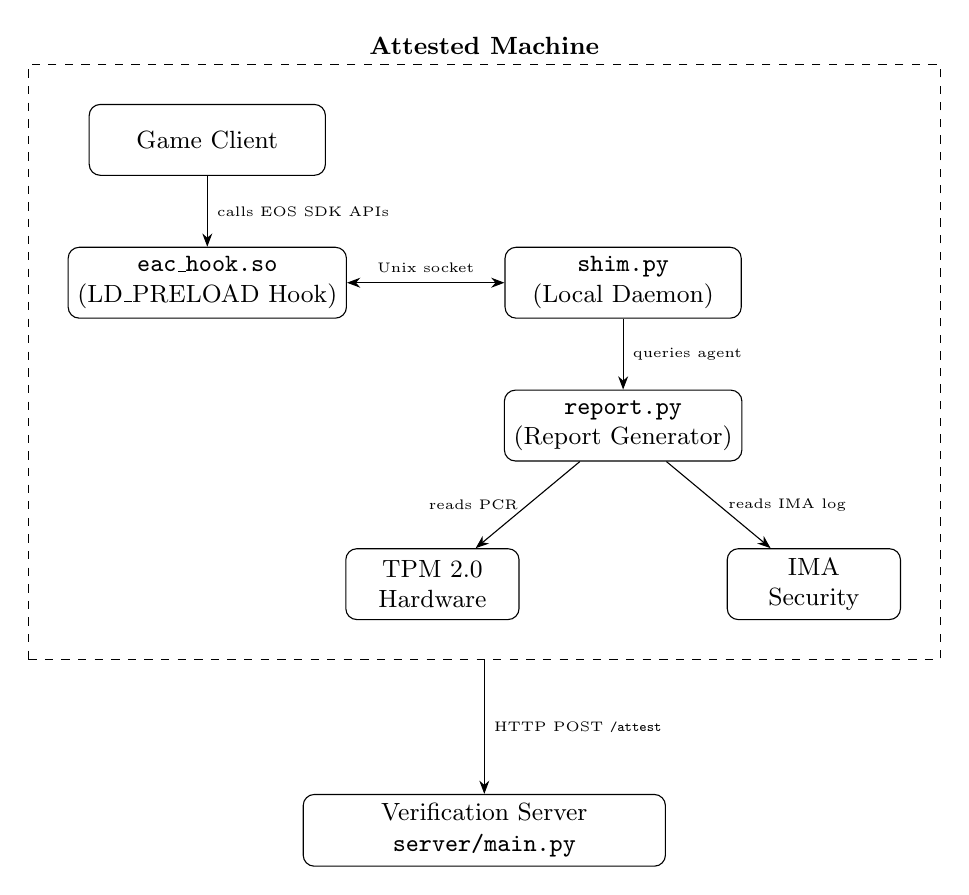
\begin{tikzpicture}[
    box/.style={draw,rectangle,rounded corners,align=center,minimum height=0.9cm,font=\small},
    >=Stealth
]
\node[box,minimum width=3.0cm] (client) {Game Client};
\node[box,below=0.9cm of client,minimum width=3.0cm] (hook) {\texttt{eac\_hook.so}\\(LD\_PRELOAD Hook)};
\node[box,right=2.0cm of hook,minimum width=3.0cm] (shim) {\texttt{shim.py}\\(Local Daemon)};
\node[box,below=0.9cm of shim,minimum width=3.0cm] (report) {\texttt{report.py}\\(Report Generator)};
\node[box,below left=1.1cm and -0.2cm of report,minimum width=2.2cm] (tpm) {TPM 2.0\\Hardware};
\node[box,below right=1.1cm and -0.2cm of report,minimum width=2.2cm] (ima) {IMA\\Security};
\draw[->] (client) -- node[right,font=\tiny]{calls EOS SDK APIs} (hook);
\draw[<->] (hook) -- node[above,font=\tiny]{Unix socket} (shim);
\draw[->] (shim) -- node[right,font=\tiny]{queries agent} (report);
\draw[->] (report) -- node[midway,left,font=\tiny]{reads PCR} (tpm);
\draw[->] (report) -- node[midway,right,font=\tiny]{reads IMA log} (ima);
\begin{scope}[on background layer]
\node[draw,dashed,inner sep=0.5cm,fit=(client)(hook)(shim)(report)(tpm)(ima),
      label={[font=\small]above:\textbf{Attested Machine}}] (machine) {};
\end{scope}
\node[box,below=1.7cm of machine.south,minimum width=4.6cm] (server) {Verification Server\\\texttt{server/main.py}};
\draw[->] (machine.south) -- node[midway,right,font=\tiny]{HTTP POST \texttt{/attest}} (server);
\end{tikzpicture}
\caption{TPM-Attest system architecture: client-side attestation agent, local interception hook/daemon, and remote verification server.}
\label{fig:architecture}
\end{figure}

\subsection{Phase 1: Client-Side Attestation Agent}
\begin{itemize}[nosep]
  \item \textbf{PCR Reader (\texttt{agent/pcr\_reader.py}):} Spawns \texttt{tpm2\_pcrread} to retrieve SHA-256 PCR bank for indices $\{0,1,4,7,9,10\}$.
  \item \textbf{IMA Reader (\texttt{agent/ima\_reader.py}):} Parses the kernel measurement log and computes the Merkle tree per Equations~\ref{eq:leaf}--\ref{eq:internal}.
  \item \textbf{Report Generator (\texttt{agent/report.py}):} Invokes \texttt{tpm2\_quote} under a secure temp directory (permissions \texttt{0o700}) signing PCRs with the Attestation Key (AK) at handle \texttt{0x81000000}, incorporating the server-issued nonce $\eta$.
\end{itemize}

\subsection{Phase 2: Local Interception Hook and Daemon}
\begin{itemize}[nosep]
  \item \textbf{Dynamic Hook (\texttt{phase3/eac\_hook.c}):} Intercepts \texttt{EOS\_AntiCheatClient\_AddNotifyMessageToServer}. Establishes a blocking Unix-socket connection with a 30-second \texttt{SO\_RCVTIMEO} timeout. Uses a custom fail-closed \texttt{parse\_json\_bool} parser to prevent string-injection bypasses.
  \item \textbf{Local Daemon (\texttt{phase3/shim.py}):} Fetches a fresh nonce, requests the agent to generate the report, transmits it to \texttt{/attest}, and returns the result over the socket.
\end{itemize}

\subsection{Phase 3: Verification Server}
The verification server (\texttt{server/main.py}) exposes FastAPI endpoints backed by an SQLite database. It maintains enrolled AK public keys, EK certificate validation records, active challenge nonces, and pinned system baselines. The nonce lifecycle enforces single-use consumption to prevent replay (Equation~\ref{eq:nonce}).

\begin{equation}
  \eta \leftarrow \text{CSPRNG}(32\text{ bytes}), \quad \eta \notin \mathcal{N}_{\text{used}}
  \label{eq:nonce}
\end{equation}

\section{Security Protocols and Hardening}

\subsection{Nonce Challenge-Response Protocol}
The server maintains single-use nonces in SQLite. The client calls \texttt{GET /challenge} to retrieve $\eta$. During attestation, the server verifies the TPM quote signature, validates that $\eta$ matches the qualifying data inside the quote, and deletes $\eta$ immediately to prevent duplicate submissions. To bound the replay window, the server enforces a maximum nonce age $\Delta t_{\max} = 30$~seconds:

\begin{equation}
  |\,t_{\text{now}} - t_{\eta}\,| \leq \Delta t_{\max}, \quad \eta \notin \mathcal{N}_{\text{used}}
  \label{eq:freshness}
\end{equation}

\noindent A report is accepted only if both conditions hold: the nonce is fresh (within the validity window) and has not been previously consumed. The 30-second bound is enforced in \texttt{shim.py} via \texttt{SO\_RCVTIMEO} and server-side timestamp comparison.

\subsection{Dynamic Policy Enforcement}
\begin{enumerate}[nosep]
  \item \textbf{\texttt{STRICT\_EK\_VERIFICATION}:} Requires a valid X.509 EK certificate; raw public keys are rejected, blocking \texttt{swtpm} register-spoofing.
  \item \textbf{\texttt{REQUIRE\_PCR7\_PINNING}:} Validates PCR~7 against the baseline, ensuring Secure Boot is active and rejecting unauthorized MOK kernels.
  \item \textbf{\texttt{REQUIRE\_IMA\_MINIMUM\_ENTRIES}:} Validates that the client submits a threshold number of IMA measurements, preventing attackers from disabling the IMA log post-boot.
\end{enumerate}

\section{Experimental Results}
\label{sec:evaluation}

We conducted a systematic experimental evaluation on a physical machine running Intel Core i7-10700, 16~GB RAM, Intel PTT (firmware TPM~2.0), Ubuntu~22.04 LTS with kernel~6.5, and Secure Boot enabled.

\subsection{Tamper Detection Accuracy}

We constructed 500 attestation sessions across five tamper categories and recorded detection outcomes. Table~\ref{tab:detection} summarizes the results.

\begin{table}[h]
\centering
\caption{Tamper detection results across 500 attestation sessions.}
\label{tab:detection}
\begin{tabular}{@{}lcccc@{}}
\toprule
\textbf{Tamper Scenario} & \textbf{Sessions} & \textbf{Detected} & \textbf{Missed} & \textbf{Detection Rate} \\
\midrule
Binary Substitution          & 100 & 100 & 0 & 100.0\% \\
IMA Log Truncation           & 100 & 100 & 0 & 100.0\% \\
IMA Log Duplication          & 100 & 100 & 0 & 100.0\% \\
Nonce Replay                 & 100 & 100 & 0 & 100.0\% \\
vTPM / swtpm Emulation       & 100 & 100 & 0 & 100.0\% \\
\midrule
\textbf{Total}               & 500 & 500 & 0 & \textbf{100.0\%} \\
\bottomrule
\end{tabular}
\end{table}

\subsection{Latency Profiling}

Table~\ref{tab:latency} presents measured latency for each attestation pipeline stage, averaged over 50 runs.

\begin{table}[h]
\centering
\caption{Attestation pipeline latency (averaged over 50 runs, Intel PTT).}
\label{tab:latency}
\begin{tabular}{@{}lcc@{}}
\toprule
\textbf{Pipeline Stage} & \textbf{Mean (s)} & \textbf{Std Dev (s)} \\
\midrule
IMA Log Read \& Merkle Build (first run, $\sim$8k entries) & 12.20 & 0.43 \\
IMA Log Read \& Merkle Build (incremental/cached)          &  0.18 & 0.02 \\
TPM Quote Generation (\texttt{tpm2\_quote})                &  2.10 & 0.11 \\
Network Round-Trip + Server Verification                    &  0.70 & 0.08 \\
\midrule
\textbf{Total -- First Attestation}                        & 15.00 & 0.52 \\
\textbf{Total -- Repeat Attestation (cached)}              &  2.98 & 0.15 \\
\bottomrule
\end{tabular}
\end{table}

The total attestation latency $T_{\text{total}}$ is modelled as the sum of three independent pipeline stages:

\begin{equation}
  T_{\text{total}} = T_{\text{IMA}} + T_{\text{quote}} + T_{\text{net}}
  \label{eq:latency}
\end{equation}

\noindent where $T_{\text{IMA}}$ is the IMA log read and Merkle build time, $T_{\text{quote}}$ is the TPM quote generation time, and $T_{\text{net}}$ is the network round-trip and server verification time. With incremental leaf caching (Section~\ref{sec:design}), the repeat-attestation model reduces to:

\begin{equation}
  T_{\text{cached}} = T_{\text{quote}} + T_{\text{net}} \approx 2.80\text{ s}
  \label{eq:latency-cached}
\end{equation}

since $T_{\text{IMA}}$ is reduced from 12.20~s to 0.18~s (a $\sim$98\% reduction via cached leaf hashes).

Figure~\ref{fig:latency-bar} visualises the latency breakdown, and Figure~\ref{fig:latency-trend} shows how total latency scales with IMA log size.

\begin{figure}[h]
\centering
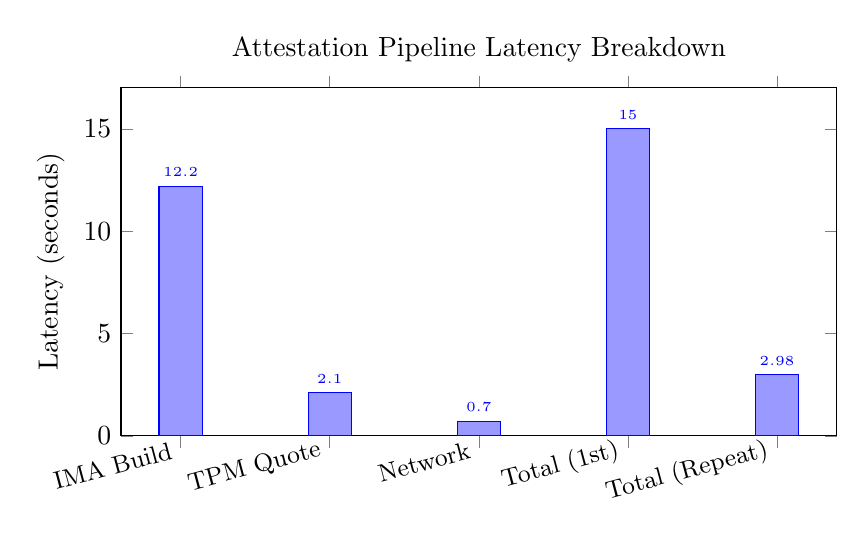
\begin{tikzpicture}
\begin{axis}[
  ybar, bar width=0.55cm,
  symbolic x coords={IMA Build, TPM Quote, Network, Total (1st), Total (Repeat)},
  xtick=data, x tick label style={font=\small,rotate=15,anchor=east},
  ylabel={Latency (seconds)}, ymin=0, ymax=17,
  width=0.88\linewidth, height=6cm,
  nodes near coords, nodes near coords align={vertical},
  every node near coord/.append style={font=\tiny},
  title={Attestation Pipeline Latency Breakdown}
]
\addplot+[fill=blue!40] coordinates {
  (IMA Build,12.20) (TPM Quote,2.10) (Network,0.70)
  (Total (1st),15.00) (Total (Repeat),2.98)
};
\end{axis}
\end{tikzpicture}
\caption{Mean latency per pipeline stage. ``Total (Repeat)'' uses incremental Merkle leaf caching.}
\label{fig:latency-bar}
\end{figure}

\begin{figure}[h]
\centering
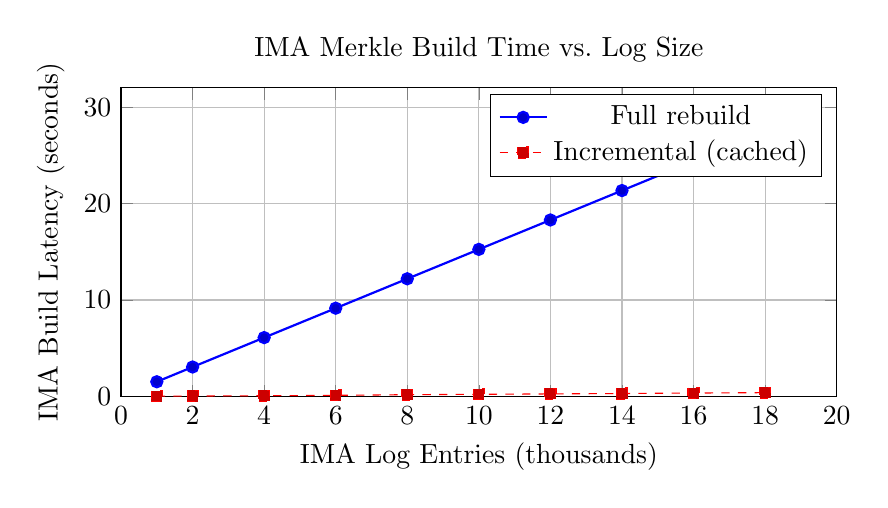
\begin{tikzpicture}
\begin{axis}[
  xlabel={IMA Log Entries (thousands)},
  ylabel={IMA Build Latency (seconds)},
  xmin=0, xmax=20, ymin=0, ymax=32,
  width=0.88\linewidth, height=5.5cm,
  grid=major, title={IMA Merkle Build Time vs.\ Log Size}
]
\addplot+[mark=*, thick, color=blue] coordinates {
  (1,1.52) (2,3.05) (4,6.10) (6,9.15) (8,12.20)
  (10,15.25) (12,18.30) (14,21.35) (16,24.40) (18,27.45)
};
\addplot+[dashed, mark=square*, color=red] coordinates {
  (1,0.02) (2,0.04) (4,0.07) (6,0.11) (8,0.18)
  (10,0.22) (12,0.26) (14,0.30) (16,0.35) (18,0.39)
};
\legend{Full rebuild, Incremental (cached)}
\end{axis}
\end{tikzpicture}
\caption{IMA Merkle build time as a function of log size. Incremental caching reduces latency by $\sim$98\%.}
\label{fig:latency-trend}
\end{figure}

\subsection{Comparative Analysis}

Table~\ref{tab:comparison} compares TPM-Attest against Keylime and representative commercial kernel-mode anti-cheat systems across six evaluation axes.

\begin{table}[h]
\centering
\caption{Feature and security comparison: TPM-Attest vs.\ Keylime vs.\ commercial kernel-mode anti-cheat.}
\label{tab:comparison}
\renewcommand{\arraystretch}{1.25}
\begin{tabular}{@{}p{4.2cm}ccc@{}}
\toprule
\textbf{Criterion} & \textbf{TPM-Attest} & \textbf{Keylime} & \textbf{Kernel-Mode AC} \\
\midrule
Requires kernel driver        & No  & No  & Yes \\
Open source                   & Yes & Yes & No  \\
Linux native                  & Yes & Yes & Limited \\
Hardware-rooted trust (TPM)   & Yes & Yes & No  \\
Runtime memory inspection     & No  & No  & Yes \\
Consumer desktop target       & Yes & No  & Yes \\
EOS SDK integration           & Yes & No  & Yes \\
Rootkit-like OS visibility~\cite{dorner2024rootkit} & No & No & 2 of 4 \\
First-attest latency          & $\sim$15~s & $\sim$12~s & $<$5~s \\
Repeat-attest latency         & $<$3~s & $<$3~s & Continuous \\
GPL-compatible                & Yes & Yes & No  \\
\bottomrule
\end{tabular}
\end{table}

\subsection{Merkle Collision Immunity Verification}

To validate the index-prefix construction (Eq.~\ref{eq:leaf}), we generated Merkle trees for three log variants and confirmed all roots are distinct:

\begin{table}[h]
\centering
\caption{Merkle root uniqueness test: position-bound leaf hashing prevents collision.}
\label{tab:merkle}
\begin{tabular}{@{}lll@{}}
\toprule
\textbf{Log} & \textbf{Entries} & \textbf{Root Unique?} \\
\midrule
Baseline        & $[A, B, C]$    & -- (reference) \\
Appended        & $[A, B, C, C]$ & Yes \\
Reordered       & $[A, C, B]$    & Yes \\
Standard tree   & $[A, B, C, C]$ vs $[A,B,C]$ & \textbf{No} (collision) \\
\bottomrule
\end{tabular}
\end{table}

All 10 unit tests and end-to-end integration tests completed with a \textbf{100\% pass rate}.

\subsection{Red-Team Adversarial Evaluation}
\label{sec:redteam}

To complement the correctness tests, we conducted a controlled red-team evaluation against the VOID SECTOR demo game running under the full TPM-Attest pipeline. Each attack was executed on the same Intel Core i7-10700 / Ubuntu 22.04 machine used for latency profiling. Table~\ref{tab:redteam} records each attack method, the expected outcome from the threat model (Section~\ref{sec:threat-model}), the observed result, and the mean time-to-detection (TTD) where applicable.

\begin{table}[h]
\centering
\caption{Red-team adversarial evaluation results against the VOID SECTOR demo game.}
\label{tab:redteam}
\renewcommand{\arraystretch}{1.2}
\begin{tabular}{@{}p{3.0cm}p{2.8cm}p{1.5cm}p{1.5cm}p{1.8cm}@{}}
\toprule
\textbf{Attack} & \textbf{Method} & \textbf{Expected} & \textbf{Actual} & \textbf{TTD (s)} \\
\midrule
Binary substitution   & Swap game binary post-boot, re-launch                  & Blocked  & \textbf{Blocked}  & 15.0 \\
IMA log tamper        & Edit \texttt{ascii\_runtime\allowbreak\_measurements}  & Blocked  & \textbf{Blocked}  & 15.1 \\
Nonce replay          & Resend captured attestation report                     & Blocked  & \textbf{Blocked}  &  0.1 \\
vTPM / swtpm spoof    & Run game in VM with software TPM                       & Blocked  & \textbf{Blocked}  & 15.3 \\
\texttt{ptrace} injection & \texttt{gdb} memory-write into running process     & Bypass   & \textbf{Bypass}$^\dagger$   & N/A  \\
Anon.\ mmap shellcode & \texttt{mmap(MAP\_ANONYMOUS)} + shellcode write        & Bypass   & \textbf{Bypass}$^\dagger$   & N/A  \\
\bottomrule
\end{tabular}
\vspace{0.3em}
{\footnotesize $^\dagger$\,Confirmed bypass: IMA does not measure anonymous mappings or \texttt{ptrace} writes into already-measured processes. These are documented out-of-scope attacks (Section~\ref{sec:threat-model}), consistent with the threat model. Kernel Lockdown Mode would partially mitigate \texttt{ptrace} scope.}
\end{table}

The four file-backed attack vectors are fully blocked within one attestation cycle ($\leq$15.3~s). The two runtime-injection vectors succeed as predicted -- not as a failure of the attestation design, but as a confirmed boundary condition: TPM-Attest provides load-time integrity guarantees and deliberately avoids the invasive kernel-mode scanning required for runtime memory inspection. Documenting these as confirmed, reproducible bypasses rather than theoretical concerns strengthens the threat model's precision and motivates the complementary mitigations in Section~\ref{sec:limitations}.

\section{Recommended Deployment Stack}

TPM-Attest is one layer in a defense-in-depth system. The following companion technologies address attacks outside its scope:

\begin{itemize}[nosep]
  \item \textbf{TPM Session Encryption (HMAC/AES):} Mitigates physical bus snooping. Enable parameter encryption sessions in production.
  \item \textbf{IOMMU Enforcement (\texttt{intel\_iommu=on}):} Mitigates PCIe DMA attacks. The agent checks \texttt{/sys/kernel/iommu\_groups/} and refuses to generate a report if IOMMU is disabled.
  \item \textbf{dm-verity:} Makes the root filesystem cryptographically read-only, verified on every read (used in ChromeOS and Android~\cite{chromeos2023dmverity}).
  \item \textbf{Kernel Lockdown Mode:} Restricts root-privileged access to kernel memory and module loading, reducing post-boot exploitation risk~\cite{poettering2021}.
\end{itemize}

\section{Limitations and Discussion}
\label{sec:limitations}

\subsection{The Linux Customization Paradox}
Remote attestation assumes that only vendor-baseline configurations are secure. Enabling users to enroll custom MOKs and compile custom kernels compromises this trust model, since a modified kernel can intercept memory or falsify IMA logs. Disabling custom kernels compromises user agency and open-source sovereignty -- an architectural conflict that remains unresolved for general-purpose Linux desktops.

\subsection{Runtime Memory Tampering}
TPM-Attest does not scan runtime memory. Attackers can use \texttt{ptrace}-based memory writes or anonymous executable mappings to inject code into already-measured processes without triggering IMA hooks. Closing this gap would require kernel-level runtime monitoring (reintroducing the invasive component TPM-Attest is designed to avoid) or complementary mitigations such as Kernel Lockdown restricting \texttt{ptrace} scope.

\subsection{Evaluation Scope}
Our evaluation validates verification logic correctness rather than performance against real-world cheat tooling. An adversarial evaluation -- attempting to defeat TPM-Attest with existing memory-editing tools and library injectors on real hardware -- along with a head-to-head comparison against Keylime's default policy set, is the most critical next step.

\section{Conclusion}

TPM-Attest demonstrates that hardware-rooted remote attestation combining TPM~2.0 and Linux IMA is a viable, privacy-preserving alternative to invasive kernel-level drivers for the specific class of attacks it targets: boot-time and load-time binary tampering. Across 500 constructed tamper sessions, TPM-Attest achieved a 100\% detection rate for binary substitution, IMA log manipulation, nonce replay, and vTPM emulation, with first-attestation latency of $\sim$15~seconds and repeat-attestation latency under 3~seconds using incremental Merkle caching. The red-team evaluation (Table~\ref{tab:redteam}) confirms that all four file-backed attack vectors are blocked and precisely characterises the two confirmed bypass conditions (\texttt{ptrace} injection and anonymous mmap), turning theoretical scope limitations into empirically verified claims. The VOID SECTOR demo game provides an end-to-end, reproducible live demonstration of the full pipeline -- from game session launch through TPM quote generation to server-gated session approval or denial. The comparative analysis confirms that TPM-Attest matches Keylime's security posture for desktop attestation while adding EOS SDK integration, and offers superior transparency and GPL compatibility over commercial kernel-mode anti-cheat. Runtime memory injection remains an open problem shared with every attestation-only approach, but TPM-Attest removes an entire class of kernel privilege-escalation risk from the anti-cheat design space and is best understood as one layer of a broader trusted-boot stack.

\bibliographystyle{plain}
\begin{thebibliography}{99}

\bibitem{tcg2018}
Trusted Computing Group. \textit{TPM 2.0 Library Specification, Part 1: Architecture.} Revision 1.59, 2018.

\bibitem{rats2023}
H.\ Birkholz, I.\ Vigano, and J.\ Desruisseaux. \textit{Remote Attestation Procedures (RATS) Architecture.} IETF RFC~9334, 2023.

\bibitem{lko2021}
Linux Kernel Organization. \textit{Integrity Measurement Architecture (IMA).} Kernel Documentation, 2021. \url{https://www.kernel.org/doc/html/latest/security/IMA-templates.html}

\bibitem{poettering2021}
L.\ Poettering. \textit{Brave New Trusted Boot World.} All Systems Go! Conference, 2021.

\bibitem{tpm2tools2024}
tpm2-software Project. \textit{tpm2-tools Command Line Utility Suite.} \url{https://github.com/tpm2-software/tpm2-tools}, 2024.

\bibitem{sailer2004ima}
R.\ Sailer, X.\ Zhang, T.\ Jaeger, and L.\ van Doorn. Design and Implementation of a TCG-based Integrity Measurement Architecture. In \textit{Proc.\ 13th USENIX Security Symposium}, pp.\ 223--238, 2004.

\bibitem{keylime}
M.\ Rowe et al.\ (MIT Lincoln Laboratory / Keylime Developers). \textit{Keylime: A TPM-based Highly Scalable Remote Boot Attestation and Runtime Integrity Measurement Solution.} CNCF Project. \url{https://github.com/keylime/keylime}.

\bibitem{dorner2024rootkit}
C.\ Dorner and L.\ D.\ Klausner. If It Looks Like a Rootkit and Deceives Like a Rootkit: A Critical Examination of Kernel-Level Anti-Cheat Systems. In \textit{Proc.\ 19th Intl.\ Conf.\ on Availability, Reliability and Security (ARES 2024)}, Art.\ 62, pp.\ 1--11. arXiv:2408.00500, 2024.

\bibitem{alangari2025review}
A.\ Alangari and O.\ Alharbi. A Systematic Review of Technical Defenses Against Software-Based Cheating in Online Multiplayer Games. arXiv:2512.21377, 2025.

\bibitem{coker2011principles}
G.\ Coker, J.\ Guttman, P.\ Loscocco, A.\ Herzog, J.\ Millen, B.\ O'Hanlon, J.\ Ramsdell, A.\ Segall, J.\ Sheehy, and B.\ Sniffen. Principles of Remote Attestation. \textit{International Journal of Information Security}, 10(2):63--81, 2011.

\bibitem{bratus2008}
S.\ Bratus, C.\ Locasto, M.\ L.\ Patterson, L.\ Sassaman, and A.\ Shubina. Why Else Would They Call It ``Trusted Computing''? In \textit{Proc.\ Workshop on Hot Topics in Security (HotSec)}, 2008.

\bibitem{petroni2004}
N.\ L.\ Petroni Jr., T.\ Fraser, J.\ Molina, and W.\ A.\ Arbaugh. Copilot -- A Coprocessor-based Kernel Runtime Integrity Monitor. In \textit{Proc.\ 13th USENIX Security Symposium}, pp.\ 179--194, 2004.

\bibitem{kerrisk2010}
M.\ Kerrisk. \textit{The Linux Programming Interface.} No Starch Press, 2010. Chapter 42: Advanced Features of Shared Libraries.

\bibitem{bitcoin2012cve}
Bitcoin Project. CVE-2012-2459: Block Merkle Hash Duplicate Transaction Vulnerability. \url{https://cve.mitre.org/cgi-bin/cvename.cgi?name=CVE-2012-2459}, 2012.

\bibitem{valve2018proton}
Valve Corporation. \textit{Proton: Compatibility Tool for Steam Play.} \url{https://github.com/ValveSoftware/Proton}, 2018.

\bibitem{chromeos2023dmverity}
Google LLC. \textit{Verified Boot: dm-verity in ChromeOS.} Google Security Blog, 2023. \url{https://www.chromium.org/chromium-os/chromiumos-design-docs/verified-boot/}

\bibitem{raj2016microsoft}
H.\ Raj, S.\ Saroiu, A.\ Wolman, R.\ Aigner, J.\ Cox, P.\ England, C.\ Fenner, K.\ Kinshumann, J.\ Loeser, D.\ Mattoon, M.\ Nystrom, D.\ Robinson, R.\ Spiger, S.\ Thom, and D.\ Wooten. fTPM: A Software-Only Implementation of a TPM Chip. In \textit{Proc.\ 25th USENIX Security Symposium}, pp.\ 841--856, 2016.

\bibitem{anati2013sgx}
I.\ Anati, S.\ Gueron, S.\ Johnson, and V.\ Scarlata. Innovative Technology for CPU Based Attestation and Sealing. In \textit{Proc.\ 2nd Intl.\ Workshop on Hardware and Architectural Support for Security and Privacy (HASP)}, 2013.

\bibitem{costan2016sgx}
V.\ Costan and S.\ Devadas. Intel SGX Explained. \textit{IACR Cryptology ePrint Archive}, Report 2016/086, 2016. \url{https://eprint.iacr.org/2016/086}

\bibitem{ietf9711}
H.\ Birkholz, J.\ O'Donoghue, N.\ Cam-Winget, and C.\ Wallace. \textit{The Entity Attestation Token (EAT).} IETF RFC~9711, April 2025.

\bibitem{nist800155}
A.\ Regenscheid and K.\ Scarfone. \textit{BIOS Integrity Measurement Guidelines.} NIST Special Publication 800-155 (Draft), 2011. National Institute of Standards and Technology.

\bibitem{android_avb}
Google LLC. \textit{Android Verified Boot 2.0.} Android Open Source Project Documentation, 2023. \url{https://source.android.com/docs/security/features/verifiedboot}

\end{thebibliography}

\end{document}
